%; whizzy chapter
% -initex iniptex -latex platex -format platex -bibtex jbibtex -fmt fmt
% 以上 whizzytex を使用する場合の設定。

%     Tokyo Debian Meeting resources
%     Copyright (C) 2011 Junichi Uekawa

%     This program is free software; you can redistribute it and/or modify
%     it under the terms of the GNU General Public License as published by
%     the Free Software Foundation; either version 2 of the License, or
%     (at your option) any later version.

%     This program is distributed in the hope that it will be useful,
%     but WITHOUT ANY WARRANTY; without even the implied warranty of
%     MERCHANTABILITY or FITNESS FOR A PARTICULAR PURPOSE.  See the
%     GNU General Public License for more details.

%     You should have received a copy of the GNU General Public License
%     along with this program; if not, write to the Free Software
%     Foundation, Inc., 51 Franklin St, Fifth Floor, Boston, MA  02110-1301 USA

%  preview (shell-command (concat "evince " (replace-regexp-in-string "tex$" "pdf"(buffer-file-name)) "&"))
% 画像ファイルを処理するためにはebbを利用してboundingboxを作成。
%(shell-command "cd image201101; ebb *.png")

%%ここからヘッダ開始。

\documentclass[mingoth,a4paper]{jsarticle}
\usepackage{monthlyreport}

% 日付を定義する、毎月変わります。
\newcommand{\debmtgyear}{2011}
\newcommand{\debmtgmonth}{2}
\newcommand{\debmtgdate}{19}
% (+ (* (- 2010 2005) 12) 10) started from zero
\newcommand{\debmtgnumber}{73}

\begin{document}

\begin{titlepage}
\thispagestyle{empty}
% タイトルページ:編集必要な部分は最初のマクロに飛ばすこと

\vspace*{-2cm}
第\debmtgnumber{}回 東京エリア Debian 勉強会資料\\
\hspace*{-2cm}
\includegraphics[width=210mm]{image201003/debsen.eps}\\
\hfill{}\debmtgyear{}年\debmtgmonth{}月\debmtgdate{}日

% ここはアップデートすること
\rotatebox{10}{\fontsize{32}{32} {\gt 特集1: Debian Games Team体験記}}

\rotatebox{10}{\fontsize{32}{32} {\gt 特集2: Squeezeリリース!みんなで語
 ろう!}}

\vspace*{-2cm}
\hfill{}
\includegraphics[height=6cm]{image200502/openlogo-nd.eps}
\end{titlepage}

\dancersection{Introduction}{上川 純一}

\begin{multicols}{2}
 

 今月のDebian勉強会へようこそ。これからDebianの世界にあしを踏み入れると
 いう方も、すでにどっぷりとつかっているという方も、月に一回Debianについ
 て語りませんか?

 Debian勉強会の目的は下記です。

 \begin{itemize}
 \item \underline{Debian Developer} (開発者)の育成。
 \item 日本語での「\underline{開発に関する情報}」を整理してまとめ、アップデートする。
 \item \underline{場}の提供。
 \begin{itemize}
  \item 普段ばらばらな場所にいる人々が face-to-face で出会える場を提供
	する。
  \item Debian のためになることを語る場を提供する。
  \item Debianについて語る場を提供する。
 \end{itemize}
 \end{itemize}		

 Debianの勉強会ということで究極的には参加者全員がDebian Packageをがりがり
 と作るスーパーハッカーになった姿を妄想しています。情報の共有・活用を通し
 て Debianの今後の能動的な展開への土台として、「場」としての空間を提供す
 るのが目的です。

\end{multicols}

\newpage

\begin{minipage}[b]{0.2\hsize}
 \definecolor{titleback}{gray}{0.9}
 \colorbox{titleback}{\rotatebox{90}{\fontsize{80}{80} {\gt デビアン勉強会} }}
\end{minipage}
\begin{minipage}[b]{0.8\hsize}
\hrule
\vspace{2mm}
\hrule
\begin{multicols}{2}
\tableofcontents
\end{multicols}
\vspace{2mm}
\hrule
\end{minipage}

\dancersection{事前課題}{上川 純一}

今回の事前課題は以下です:
\begin{enumerate}
 \item ヤッター、リリースしたよ! Squeezeになってうれしいこと、Squeezeになって変わったことを教えてください。
\end{enumerate}
この課題に対して提出いただいた内容は以下です。
\begin{multicols}{2}
{\small
 %; whizzy-master ../debianmeetingresume201101.tex
% $B0J>e$N@_Dj$r$7$F$$$k$?$a!"$3$N%U%!%$%k$G(B M-x whizzytex $B$9$k$H!"(Bwhizzytex$B$,MxMQ$G$-$^$9!#(B

\begin{prework}{ $B%-%?%O%i(B }

$B<B2H$K%j%j!<%9A0$N(BSqueeze$B$rCV$$$F$-$?$,!"FC$KLdBj$J$/;HMQ$5$l$F$$$kMM;R!#(B
$B2?$b@_Dj$7$J$/$F$b!"%5%9%Z%s%I!&%O%$%P%M!<%7%g%s$G$-$?$h$&$J!"%W%j%s%?$N@_Dj$K>/!9G:$s$@5-21$,$"$k$,!">\:Y$OK:$l$?!#(B
$B@N$KHf$Y$k$H3JCJ$K3Z$K$J$j$^$7$?!#(B
\end{prework}

\begin{prework}{ $B5HLn(B(yy\_y\_ja\_jp) }

poppler-data,cmap-adobe-*,gs-cjk-resource $B$,(B main $B$KF~$C$?$3$H$G$9$M!$(BThanks to Adobe$B!%(B
\end{prework}

\begin{prework}{ d123.itouch.com(dai) }

 \begin{itemize}
  \item $B1'Ch$,%F!<%^$G$+$C$3$$$$!*(B
  \item $B?7$7$/(BDebian$B$r3P$($k$3$H$K$J$C$?$N$G!"CzEY$$$$5!2q$G$9!#(BDebian$B=i(B
	$B?4<T!*0lG/@8$G$9!*(B
 \end{itemize}

 2$BG/$[$IA0$KEl5~$NK?@lLg3X9;$G3+:E$5$l$?5.2q$N%V!<%9$G$4CzG+$K(B
 $B$4>R2p$$$?$@$$$?$3$H$,$"$j$^$9!#$9$P$i$7$$2q$r3+:E$$$?$@$-(B
 $B$"$j$,$H$&$4$6$$$^$9!#:#2s=i$N;22C$G$9!#$I$&$>$h$m$7$/$*4j$$$7$^$9!#(B
\end{prework}

\begin{prework}{ hakase }

$B$9$$$^$;$s!"(BSqueeze$B$NL>A0;O$a$FJ9$-$^$7$?!#(B
$BJY6/$7$^$9!#(B
\end{prework}

\begin{prework}{ henrich }

$B$9$$$^$;$s!"FCCJ8D?ME*$K$&$l$7$$$H$3$m$,8+Ev$?$j$^$;$s$G$7$?!D(B
\end{prework}

\begin{prework}{ $B;3ED(B }

\preworksection{$B$&$l$7$$$3$H(B}
\begin{itemize}
 \item /bin/sh$B$,(Bdash$B$K$J$C$?!*%9%/%j%W%H5/F0$,L@$i$+$K7Z$$(B
 \item $B0MB84X78%Y!<%9$G5/F0=hM}$,$5$l$k$h$&$K$J$C$?!JAa$/$J$C$?!K(B
 \item $B%Q%C%1!<%8$,$5$i$K=<<B$7$?!J5$$E$$$F$J$+$C$?$@$1$+$b$7$l$J$$$b$N$N!"!V$3$s$J$N$^$GF~$C$F$k!WEY$,>e>:!K(B
 \item $B%j%j!<%9%9%1%8%e!<%k$,$7$C$+$j$7$F$-$?(B
\end{itemize}

\preworksection{$BJQ$o$C$?$3$H!J5$$K$J$k$3$H!K(B}
\begin{itemize}
 \item kFreeBSD$B$,F~$C$?!*$9$0;H$&$o$1$G$O$J$$$1$I!"5$$K$J$k(B
 \item arm(eb)$B$,Mn$C$3$A$?$1$I!"@$$NCfBgBN(Barmel$B$@$+$i(BOK$B$J$N$+$J!)(B
 \item Debian Live$B!#(BLiveCD$B$+$i(Bnetboot$B$^$G%+%P!<$H$$$&$3$H$GMW%A%'%C%/(B
\end{itemize}
$B%j%j!<%9$NA0$+$i<B:]$K$O;H$($F$$$?$N$G!V@hF|$+$i$$$-$J$j$&$l$7$/$J$C$?!W;v$O<B$O$J$$$b$N$N!"Ce<B$J%j%j!<%9$H$$$&46A[$G$9!#(B
\end{prework}

\begin{prework}{ dictoss($B?yK\!!E5=<(B) }

$B5/F0$,Aa$/$J$C$?!#(B
Debian GNU/kFreeBSD$B$NL>$,9-$^$C$F$-$?!#(B
\end{prework}

\begin{prework}{ yamamoto }

\preworksection{$B$&$l$7$$$3$H(B}
Squeeze $B$@$+$i!"$H$$$&$o$1$G$O$J$$$G$9$,!"(Bdebian-multimedia $B$N(B mythtv $B$,(B
 0.24 $B7O$K$J$C$F!"(Bmythtv-backend $B$,FMA3;`$9$k$3$H$,L5$/$J$j$^$7$?!#(B

\preworksection{$BJQ$o$C$?$3$H(B}
KDE $B$r>oMQ$7$F$^$9$,!"(BKlipper $B$N5sF0$,JQ$o$C$?!#$J$s$+;~!9!"$o$6$o$6(B Klipper $B$N%A%'%C%/$r$D$1$J$$$H!"Cf%\%?%s$GA*BrJ8;zNs$r%Z!<%9%H$G$-$J$$!#(B
$B860xD4::$O$^$@$@$1$I!D!#(B
$B!V%/%j%C%W%\!<%I$N%"%/%7%g%s$rM-8z$K$9$k!W$"$?$j$,$"$d$7$$(B!?
\end{prework}

\begin{prework}{ $BLnEg!!5.1Q(B }

$B$&$O$C!"IaCJ$+$i(Bunstable(sid)$B$7$+;H$C$F$J$$(B...

$B<h$j5^$.(Blenny$B$H$N0c$$$G4r$7$$;v!#(B
\begin{enumerate}
 \item kernel$B$,(B2.6.32$B7ONs$K$J$C$?!#(B(kvm$B$N%P!<%8%g%s$,>e$,$C$?!*(B)
 \item libvirt$B$,(B0.8.3$B$K$J$C$?!#!J$$$m$s$J%Q%i%a%?$,$$$m$$$m$D$1J|Bj$K(B...)
 \item gnome$B$,(B2.30$B7ONs$K$J$C$?!#(Bfreedesktop-sound-theme$B$,I8=`AuHw$5$l$?$N$G2;$,$K$.$d$+$K$J$C$?!#(B
 \item upstart$B$,Ek:\$5$l$?!#(B(sid$B;H$C$F$$$k$N$G$9$,!"(Bupstart$B$K$J$C$F$J$/(B
       $B$F$,$C$/$j!#:#$+$iJQ$($F$_$^$9(B...)
\end{enumerate}
\end{prework}

\begin{prework}{ taitioooo }

$B=i$a$F(BDebian$B$K?($C$?$N$,(Bsqueeze$B$G$7$?!#(B
$B:#$^$G(BCentos$B;H$C$F$$$^$7$?!#(B
$B=i$a$F$N0u>]$O!"!V$"!"%m%1%C%H$,$"$k!#!W$G$7$?!#(B

$B$"$H!"(Bapt-get$B$N@_Dj$,4JC1$G$h$+$C$?$G$9!#!J(Byum$B$HHf$Y$F$G$9$,!K(B
\end{prework}

\begin{prework}{ Hasegawa }

$B%$%s%9%H!<%k$G(Broot$B$G%m%0%$%s$9$k$+J9$$$F$-$?$j(B
$B@_Dj9`L\$,A}$($?$h$&$@$7!"$+$J$jJQ$o$C$?0u>]$r;}$C$?(B
64bit/32bit$B$,A*Br$G$-$k%$%s%9%H!<%i!<$K$J$C$?(B

\end{prework}

\begin{prework}{ ayakomuro }

$B$^$@%"%C%W%0%l!<%I$7$F$J$$$N$G!"=5Kv$K%"%C%W%0%l!<%I$7$?$i>\:Y=q$-$^$9(Bm(..)m
\end{prework}

\begin{prework}{$B$^$($@$3$&$X$$(B}

\preworksection{$B$&$l$7$$$3$H(B}
\begin{itemize}
 \item Squeeze$B$,%j%j!<%9$5$l$?$3$H$G(BSid$B$N3+H/$,:F3+$5$l$?$N$G!"(BCouchApp$B$d(B
       xserver-xorg-input-multitouch$B$,(BDebian$B%Q%C%1!<%8$K$J$C$?!#(B
 \item Sarge$B$G2TF/Cf$NAH9g%5!<%P$r%O!<%I%&%'%"!u%7%9%F%`O75`2=$K$h$j!"(B
       KVM/Squeeze/HP MicroServer$B$G9=C[Cf$J$N$G!"%j%j!<%9$5$l$F$A$g$&$I(B
       $BNI$+$C$?!#(B
 \item $B:#$^$G(BSid$B$G$7$+;H$($J$+$C$?%Q%C%1!<%8$,(Bstable$B$G;H$($k$h$&$K$J$C$?(B
       $B$b$N$,A}$($?!#(B(lxc, scala, xz-utils, libapache-mod-security($B$3$l$OI|3h$7(B
       $B$?!"$H$$$&$N$,@5$7$$$+(B))
 \item $B5/F0%9%/%j%W%H$,(Bbash$B$+$i(Bdash$B$KJQ$o$C$?!#(BVM$B$G$b5/F0$,B.$/$J$C$?5$(B
       $B$,$9$k!#(B($BBN46B.EY!#(B)
\end{itemize}
\preworksection{$BJQ$o$C$?$3$H(B}
\begin{itemize}
 \item libvirt$B$,(B0.8.3$B$K$J$C$?!#(Bnwfilter$B$N5!G=$,F~$C$?(B
       (/etc/libvirt/nwfilter/*.xml)$B!#(BNetfilter$B$N%k!<%k$O$9$Y$F<+J,$G=q(B
       $B$$$F$$$k$N$G!"<+J,$K$OI,MW$J$$$1$l$I!"IaCJ=q$+$J$$(BNetfilter$B$N%k!<(B
       $B%k$r=q$+$J$$?M$K<h$C$F$ONI$$$N$G$O!#(B
 \item $B%/%i%&%I4XO"$N%D!<%k$,%Q%C%1!<%8$GA}$($?!#;~Be$G$9$M!<!#(B
\end{itemize}
\end{prework}



}
\end{multicols}

\dancersection{最近のDebian関連のミーティング報告}{上川純一}
\subsection{東京エリアDebian勉強会72回目報告}

% (query-replace-regexp "<.*?>" "")
% (query-replace-regexp "^[	 ]\+" "")

2011年1月15日に開催しました。
参加者は前田さん、kuwa\_twさん、emasakaさん、nozzyさん、上川、本庄さん、山本さん、村田信
人さん、higashiyamaさん、キタハラさん、武藤さん、山田(泰)さんでした。

\begin{itemize}
 \item クイズ、全問正解はnozzyさんと村田信人さんでした。(多分)
 \item 事前課題は未来予想で盛り上がりました。
 \item 上川さんがDebian勉強会アンケートシステムを紹介、GNU Rを使って解析してみた例を紹介しました。
 \item 山田さんがKinectを使ったデモ、プレゼンを頑張って踊りながら制御し
       てました。
 \item 宴会は近所の「魚こう」にて。CACert Assuranceも宴会場所でやりまし
       たが、Assurerにやさしくない宴会になりました。
\end{itemize}


\dancersection{Debian Trivia Quiz}{上川 純一}

ところで、みなさん Debian 関連の話題においついていますか?Debian関連の話
題はメーリングリストをよんでいると追跡できます。ただよんでいるだけではは
りあいがないので、理解度のテストをします。特に一人だけでは意味がわからな
いところもあるかも知れません。みんなで一緒に読んでみましょう。

今回の出題範囲は\url{debian-devel-announce@lists.debian.org} や \url{debian-devel@lists.debian.org}に投稿された
内容とDebian Project Newsからです。

\begin{multicols}{2}
 %; whizzy-master ../debianmeetingresume201101.tex
% $B0J>e$N@_Dj$r$7$F$$$k$?$a!"$3$N%U%!%$%k$G(B M-x whizzytex $B$9$k$H!"(Bwhizzytex$B$,MxMQ$G$-$^$9!#(B
%
% $B$A$J$_$K!"%/%$%:$OJL%V%i%s%A$G:n@.$7!"$N$A$K%^!<%8$7$^$9!#5U$K%^!<%8$7(B
% $B$J$$$h$&$K$7$^$7$g$&!#(B
% (shell-command "git checkout quiz-prepare")

\santaku
{Debian 6.0 $B$,%j%j!<%9$5$l$?$N$O$$$D$+!)(B}
{2011/02/05}
{2011/02/06}
{2011/02/07}
{A}
{}

\santaku
{$B:#2s$N%j%j!<%9$G%5%]!<%H$5$l$J$/$J$C$?%"!<%-%F%/%A%c$O!)(B}
{m68k, ppc64}
{alpha, arm, hppa}
{blackfin, microblaze}
{B}
{}

\santaku
{www.debian.org $B$N%G%6%$%s$,JQ99$5$l$^$7$?!#2?G/F1$8%G%6%$%s$r;H$C$F$$$?$+!)(B}
{11$BG/(B}
{12$BG/(B}
{13$BG/(B}
{C}
{}

\santaku
{$B<!$N%j%j!<%9%3!<%I%M!<%`$O2?$+!)(B}
{rc}
{spell} % Mr.Spell
{wheezy}
{C}
{}

\santaku
{$B:#EY9T$o$l$k(BFTP-master$B2q5D$G5DO@$5$l$J$$M=Dj$O!)(B}
{$B%Q%C%1!<%8<+F0%5%$%s5!9=(B}
{$B%/%m%9%3%s%Q%$%k%5%]!<%H(B}
{md5sum$B$H(BshaXsum$B$r$H$C$Q$i$&(B}
{B}
{}

\santaku
{Lars Wirzenius$B$,Ds0F$7$?<!$N%j%j!<%9%4!<%kL\I8$O!)(B}
{UTF-8$B$GF0$+$J$$%Q%C%1!<%8$r$J$/$9(B}
{Debian$B$GF0$$$F$$$k?M9)1R@1$rBG$A>e$2$^$9(B}
{$BA4%Q%C%1!<%8$r(BLLVM$B$G%S%k%I$7$^$9(B}
{A}
{}

\end{multicols}


%-------------------------------------------------------------------------------
\dancersection{Debian Games Team体験記}{野島 貴英}
%-------------------------------------------------------------------------------
\index{Debian Games Team}
\index{xmris}

 ひょんな事からDebian Games Team Projectに参加してしまったドタバタの体験記となります。パッケージ初心者の初心者視点の右往左往を楽しんでいただければ幸いです。

\subsection{あれ?Xmrisが無い!?}

 学生の頃、初めて触ったライセンスFreeのUNIX(linux。当時はSlackware)で遊びまくっていたゲームに、Xmrisというのがあります。Xmrisは、当時、計算機科学の追求の為に導入されていたはずのあらゆる商用UNIXマシンに\underline{何故か必ず入っていたゲーム}でした。自分の学校とは全く無関係の施設のUNIXマシンにすら入っていたゲームだったので、思わずMIT Xの配布物に梱包されているんだとずっと誤解していたりしました。

\begin{figure}[H]
\begin{center}
 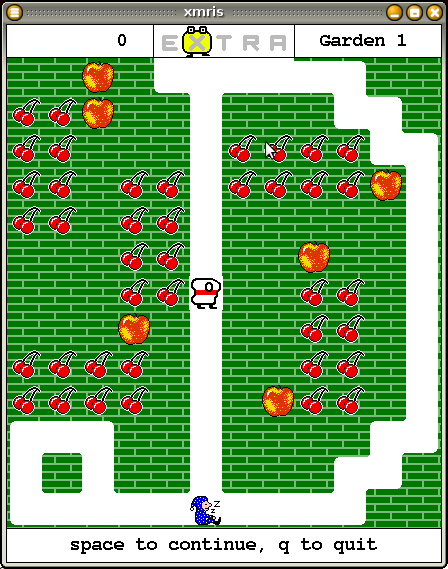
\includegraphics[height=0.5\hsize] {image201102/xmris-top.png}
 \caption{Xmirsの画面}
\label{fig:xmris-top}
\end{center}
\end{figure}

\newpage

 で、昔を懐しんでこのXmrisがやりたくなり、早速aptitude search xmrisしてみたところ、

 \begin{center}
  \Large{ごはっ、Xmrisがどこにも無いっ!?}
 \end{center}

 でした。で、「もしや?」と思い、方々捜し回ったところ、
Debian WikiのGames/Suggestedのページ
(\url{http://wiki.debian.org/Games/Suggested})のパッケージにして欲しいリストにXmirsの名前が燦然と輝いているではありませんか。


\subsection{Debian Games Teamへ}

 Xmrisがとにかくやりたかった為、完璧にパッケージ作成初心者ではありましたが、Debian Policy文章、apt-get sourceコマンド、lintianコマンドのお陰で苦労なくパッケージを作成できました。

 が、パッケージは作ったものの、当時、自分の周りにはDDは全くおらず、「どうやったらパッケージを取り込んでもらえるのだろう?」と言う事で悩みまくることになりました。で、辿り着いたのがDebian Game Teamでした。

 右も左も分からない状況で Debian Games TeamのML(\url{debian-devel-games@lists.debian.org}以下ML)でおそるおそるやり取りしたところ以下の事がわかりました。

 \begin{description}
 \item [参加資格]\mbox{}\\
   実際にGameのパッケージをつくろうとしている人はだれでも(初心者ならなおさら入って他の人のパッケージの作り方とやりとりを見てくれと言われた)
 \item [参加方法]\mbox{}\\
   こんな感じで進めます。
   \begin{description}
   \item [Step 1.]まずMLに参加したい意志表明を流す(例:これこれのパッケージを作りたいので入れて欲しい等)
   \item [Step 2.]次にalioth.debian.org(以下alioth)にアカウントを作り(\url{http://alioth.debian.org/account/register.php})、alioth上のDebian Games Teamのページ(\url{http://alioth.debian.org/projects/pkg-games/})にある``Request to join''のリンクから参加のリクエストを送る。
  \item [Step 3.] 後日Debian Games Teamの管理者からWellcomeレターが届き、alioth上のDebian Games TeamのページのProject Membersの欄に名前が登録される。
   \end{description}
 \item [実際の開発]\mbox{}\\
   マニュアル(\url{http://wiki.debian.org/Games/VCS},\url{http://wiki.debian.org/Games/VCS/git})を見てVCS/ML/IRCを活用しながらパッケージ開発を進めることになります。(IRCは、irc.debian.orgサーバー上の\#debian-gamesチャンネル)
   \begin{description}
   \item [Step 1.] マニュアルに従い作ろうとしているパッケージのリポジトリを堀る。(勝手にバンバン掘って良いとの事です)
   \item [Step 2.] gitコマンドを使ってどんどんパッケージの修正をアップロードしていく。
   \item [Step 3.] パッケージが完成したら、mentor.debian.netにアップロードして、mentorを募る。うまくmentorがつけば、Debianのパッケージリリースのプロセスにのるハズ。
   \end{description}
 \end{description}
 \newpage

\subsection{私見}

 以下にDebian Game Teamに関する私見をば。

 \begin{itemize}
 \item ゲームをdebianパッケージにしたい人が情報交換をする為に単に集まる寄合い場所のような位置づけなので、Debian Game Teamとして、ゲームのパッケージを作成する以外の明確なビジョンとかルールがあるわけではない。その為、 Debian Game Teamのエリアに自分のgitリポジトリを掘るときに「こうしていいか?ああしていいか?」といちいち許可を求めると、ウザがられるのは驚いた(最後はあなたの好きにしてくれ、本当にまずかったら指摘を受けるからその時に覚えてくれといわれてしまった。まあ、聞き方の問題だったのかもしれない...)
   \item きっとDebian Game Teamの関係者と面識が在るといろいろやりやすいと思う。
   \item Debian Game Team以外でも身の回りに相談できるDDがいると大変違う(Debianで常識、Debian Game Teamで常識をうまく切り分けられる)
   \item 規模大き目のゲームをパッケージにまとめる際、付属しているバイナリデータ群に
        別のライセンスが適用/良くわからないライセンスが適用されていることがあり、
         こちらの扱いで頭を抱える事がある。
        (キャラクタの画像、背景の画像、ゲーム内部で使われているフォント、サウンドetc...)
   \item 手のかかる問題の解決/ちょっと揉めるリスクのある問題の解決(ライセンス問題、以前のパッケージメンテナ/アップストリームに結局連絡取れない、uploadに関してスポンサーがつかない等)については、消極的。結局、こちらはパッケージメンテしようとする側にて解決が求められる。
   \item MLに流れるやりとりよりも、IRCでのやり取りの方が多い印象。また、話も早い事が多い。MLで回答が得られなくてもがっかりせず、その場合はIRCへ突撃をお勧め。
   \item 空気を読むとpackageを作成する方法、debian policyなどは基礎知識としてある事が前提。
   \item チームに所属している人の生活があふれるやり取りがIRCで日常的に行われているのは新鮮だった。例:今、「会社でたよー。ちょっとまってねー」→ 「はい家についたから繋いだよー。〜の件はねー」と会話が続く。日常生活の一部として、Contribution活動が組み込まれてしまっているのは自分にとっては感動ものでした。
 \end{itemize}

%-------------------------------------------------------------------------------
\dancersection{Hadoop本読書会報告&俺様FSを入れてみた話}{山田泰資}
%-------------------------------------------------------------------------------
\index{Hadoop}
\index{HDFS}

HadoopはTB-PB級の大規模データを複数のサーバに分散して並列処理するための
プラットフォームです。実際の所、そんな大きなデータ処理は私はしていないの
ですが、多数サーバーの制御・スケーリング処理の題材として実験に使っています。

この解説書の決定版としてオライリーから「Hadoop, The Definitive Guide」という
本が出ている(第1版は訳書も出ている)のですが、昨年半ばに第2版が出版され、
その読書会を行っています。そこではHDFS章の解説を担当したのですが、
その(アップデートされた)報告を行います。Hadoopの使い方ではなく、HDFSの
設計・動作の話になります。

また、本にはないおまけとして、HDFSではなく独自にFSを定義して、Hadoopに
組み込んでみました\footnote{本にはできるとは書いてあったものの、具体的に
書いていなかったのでやってみた}。この実験は(当然)Debianで行ったので、
その際のDebian上での手順や注意点もあわせてお話します。

なお、今回は都合のためスクリーン資料のみとなります。

%-------------------------------------------------------------------------------
\dancersection{Squeezeをみんなインストールした結果を語る会}{まえだこうへい}
%-------------------------------------------------------------------------------
\index{squeeze}

事前課題ではSqueezeになってうれしい点、変わった点を挙げてもらいましたが、
実際にインストールしてみた結果を語りましょう。

\subsection{インストールした機器}

\begin{table}[ht]
 \begin{center}
  \begin{tabular}{|p{10em}|p{15em}|p{15em}|}
   \hline
   メーカー & 機種名 & 誰 \\
   \hline
   HP & MicroServer & まえだ\\
   \hline
  \end{tabular}
 \end{center}
\end{table}

\subsection{インストールで困ったこと}

\begin{table}[ht]
 \begin{center}
  \begin{tabular}{|p{15em}|p{10em}|p{15em}|p{5em}|}
   \hline
   困ったこと & 解決したか? & 解決方法 & 担当 \\
   \hline
   プリンタの設定に少々悩んだ(詳細忘れた)& 解決? & 解決方法を思い出して情報共有す
	   る。 & キタハラ\\
   \hline
  \end{tabular}
 \end{center}
\end{table}

\subsection{改善した方が良いと思ったこと}

\begin{table}[ht]
 \begin{center}
  \begin{tabular}{|p{15em}|p{10em}|p{15em}|p{3em}|}
   \hline
   改善した方良いと思ったこと & Sidでも再現するか? & あなたの宣言 & 担
   当 \\
   \hline
   libvirt のnwfilterの設定によって、自分で設定しているiptablesのルール
   が上書きされる & 未検証 & /etc/libvirt/nwfilterにルールを追加するか、その
	   下をすべて削除して自分で作っているスクリプトに集約する。前者
	   はルールの順番がよく分からないので仕組みを理解する。 & まえだ\\
   \hline
   Klipperの挙動が変わり、中ボタンでのペースが面倒になった。& & 「クリップ
	   ボードのアクションを有効にする」で解決するか確認する。しなけ
	   れば改善案を考えてBTS。 & 山本\\
   \hline
   心残りがあること & そのままSidにある? & すっきり解決する。 & 岩松 \\
   \hline
   Debian InstallerでLVMを一度設定すると削除できない。& Yes。シェルモー
       ドでlvremove, vgremove, pvremoveすれば削除できる。 & メニューから
	   も普通に削除できた方が良いんじゃね。 & まえだ \\
   \hline
  \end{tabular}
 \end{center}
\end{table}

\printindex

\cleartooddpage

\vspace*{15cm}
\hrule
\vspace{2mm}

\includegraphics[width=2cm]{image200502/openlogo-nd.eps}
\noindent \Large \bf Debian 勉強会資料\\
\noindent \normalfont \debmtgyear{}年\debmtgmonth{}月\debmtgdate{}日 \hspace{5mm}  初版第1刷発行\\
\noindent \normalfont 東京エリア Debian 勉強会 (編集・印刷・発行)\\
\hrule

\end{document}
